\documentclass{beamer}
\usepackage{polski}
\usepackage[utf8]{inputenc}
\usepackage{graphicx}
\usetheme{Warsaw}
\author{Marcin Fabrykowski}
\title{Przyczyny katastrofy Hindenburga}
\begin{document}
\begin{frame}
\maketitle
\end{frame}
\section{Podstawowe informacje}
\subsection{Czym był Hindenburg?}
\begin{frame}
	\frametitle{Czym był Hindenburg}
	\begin{block}{Pełna nazwa}<1->
		LZ 129 Hindenburg
	\end{block}
	\begin{block}{Zastosowanie}<2->
		\begin{itemize}
			\item cywilne
			\item transport transatlantycki
		\end{itemize}
	\end{block}
\end{frame}
\subsection{Czym była seria Zeppelins?}
\begin{frame}
	\frametitle{Co znacza LZ?}
	\begin{block}{LZ}
		Luftschiff Zeppelin
	\end{block}
		\begin{block}{Zeppelin}<2->
		\begin{itemize}
			\item<3-> seria sterowców
			\item<4-> Ferdinand von Zeppelin
		\end{itemize}
	\end{block}
\end{frame}
\subsection{Czym był sterowiec?}
\begin{frame}
	\frametitle{Czym był sterowiec?}
	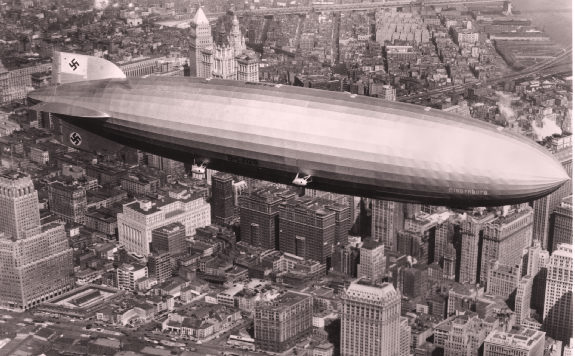
\includegraphics[width=0.8\paperwidth]{Hindenburg}
\end{frame}
\subsection{LZ 129 Hindenburg}
\begin{frame}
	\frametitle{LZ 129 Hindenburg}
	\begin{block}{wymiary}
	Długość: 245m\\
	Średnica 41m
	\end{block}
	\uncover<2->{
		\begin{center}
		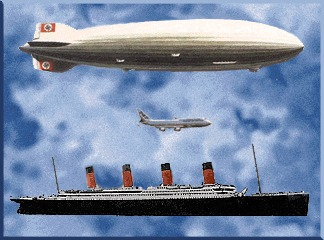
\includegraphics[width=0.5\paperwidth]{Hind_size}
		\end{center}
	}
\end{frame}
\begin{frame}
	\frametitle{LZ 129 Hindenburg}
	\begin{block}{Pojemność}
		\begin{itemize}
			\item Pasażerowie: 50 - 72
			\item Załoga: 61
		\end{itemize}
	\end{block}
	\begin{block}{Napęd}
		4x silnik diesla 1200KM
	\end{block}
	\begin{block}{Prędkość}
		Prędkość maksymalna: 135km/h
	\end{block}
\end{frame}
\end{document}
